%%
%% Copyright 2007, 2008, 2009 Elsevier Ltd
%%
%% This file is part of the 'Elsarticle Bundle'.
%% ---------------------------------------------
%%
%% It may be distributed under the conditions of the LaTeX Project Public
%% License, either version 1.2 of this license or (at your option) any
%% later version.  The latest version of this license is in
%%    http://www.latex-project.org/lppl.txt
%% and version 1.2 or later is part of all distributions of LaTeX
%% version 1999/12/01 or later.
%%
%% The list of all files belonging to the 'Elsarticle Bundle' is
%% given in the file `manifest.txt'.
%%

%% Template article for Elsevier's document class `elsarticle'
%% with numbered style bibliographic references
%% SP 2008/03/01
%%
%%
%%
%% $Id: elsarticle-template-num.tex 4 2009-10-24 08:22:58Z rishi $
%%
%%
%\documentclass[preprint,12pt]{elsarticle}

%% Use the option review to obtain double line spacing
%\documentclass[preprint,review,12pt]{elsarticle}
\documentclass[preprint,10pt]{elsarticle}

%% Use the options 1p,twocolumn; 3p; 3p,twocolumn; 5p; or 5p,twocolumn
%% for a journal layout:
%% \documentclass[final,1p,times]{elsarticle}
%% \documentclass[final,1p,times,twocolumn]{elsarticle}
%% \documentclass[final,3p,times]{elsarticle}
%% \documentclass[final,3p,times,twocolumn]{elsarticle}
%% \documentclass[final,5p,times]{elsarticle}
%% \documentclass[final,5p,times,twocolumn]{elsarticle}

%% if you use PostScript figures in your article
%% use the graphics package for simple commands
%% \usepackage{graphics}
%% or use the graphicx package for more complicated commands
%% \usepackage{graphicx}
%% or use the epsfig package if you prefer to use the old commands
%% \usepackage{epsfig}
%%%%%%%%%%%%%%%%%%%%%%%%%%%%%%%%%%%%%%%%%%%%%%%%%%%%%%%%%%%%%%%%%%%%
%% Package Listing
\usepackage{color}
\usepackage{graphicx}
\usepackage{amssymb}
\usepackage{amsmath}
\usepackage{amsfonts}
\usepackage{amstext}
\usepackage{amsbsy}
\usepackage{subcaption}
\usepackage{epstopdf}
%%%%%%%%%%%%%%%%%%%%%%%%%%%%%%%%%%%%%%%%%%%%%%%%%%%%%%%%%%%%%%%%%%%%
%% The lineno packages adds line numbers. Start line numbering with
%% \begin{linenumbers}, end it with \end{linenumbers}. Or switch it on
%% for the whole article with \linenumbers after \end{frontmatter}.
\usepackage{lineno}
%%%%%%%%%%%%%%%%%%%%%%%%%%%%%%%%%%%%%%%%%%%%%%%%%%%%%%%%%%%%%%%%%%%%
% DGFEM commands
\newcommand{\jmp}[1]{[\![#1]\!]}                     % jump
\newcommand{\mvl}[1]{\{\!\!\{#1\}\!\!\}}             % mean value
\newcommand{\keff}{\ensuremath{k_{\textit{eff}}}\xspace}
%% Other Commands
\newcommand{\tcr}[1]{\textcolor{red}{#1}}
\newcommand{\mt}[1]{\marginpar{ {\tiny #1}}}
\newcommand{\Introfigpath}[1]{../../../Document/Rev0/figures/sec_Intro/{#1}}
\newcommand{\Snfigpath}[1]{../../../Document/Rev0/figures/sec_Sn/{#1}}
\newcommand{\BFfigpath}[1]{../../../Document/Rev0/figures/sec_BF/{#1}}
\newcommand{\DSAfigpath}[1]{../../../Document/Rev0/figures/sec_DSA/{#1}}
%%%%%%%%%%%%%%%%%%%%%%%%%%%%%%%%%%%%%%%%%%%%%%%%%%%%%%%%%%%%%%%%%%%%
\journal{Nuclear Science and Engineering}

\begin{document}
%-------------------------
\begin{frontmatter}
%-------------------------
\title{Parellelizable Methodology for Accelerating Thermal Neutron Upscattering}
%-------------------------
\author{Michael W. Hackemack}
\author{Jean C. Ragusa}
\ead{jean.ragusa@tamu.edu}
\address{Department of Nuclear Engineering, Texas A\&M University, College Station, TX 77843, USA}
%-------------------------
\begin{abstract}
%% Text of abstract
abstract goes here...
\end{abstract}
%-------------------------
\begin{keyword}
Thermal Neutron Upscattering \sep Two-Grid \sep DSA \sep Parallel \sep Jacobi
\end{keyword}
%-------------------------
\end{frontmatter}
%-------------------------
%%%%%%%%%%%%%%%%%%%%%%%%%%%%%%%%%%%%%%%%%%%%%%%%%%%%%%%%%%%%%%%%%%%%

\linenumbers

%%%%%%%%%%%%%%%%%%%%%%%%%%%%%%%%%%%%%%%%%%%%%%%%%%%%%%%%%%%%%%%%%%%%
%%%%%%%%%%%%%%%%%%%%%%%%%%%%%%%%%%%%%%%%%%%%%%%%%%%%%%%%%%%%%%%%%%%%
\section{Introduction} \label{sec::intro}
%%%%%%%%%%%%%%%%%%%%%%%%%%%%%%%%%%%%%%%%%%%%%%%%%%%%%%%%%%%%%%%%%%%%
%%%%%%%%%%%%%%%%%%%%%%%%%%%%%%%%%%%%%%%%%%%%%%%%%%%%%%%%%%%%%%%%%%%%

\tcr
{
\begin{enumerate}
\item Brief description of outer-iteration scheme for multigroup problems (words only). Historically (and still used today in several software, ref, simulate ), this was a GS procedure (note: some recent works build athe full MG unsymmetric matrix, rattlesnake, parcs). Why is acceleration of GS important? D2O, C.
transition to previous work on acceleration of GS
\item Historical upscatter acceleration work:
\begin{itemize}
\item: start with TG 1993, in passing Averin+Vol., MTG, MF-grey (was this before TG?). As closing, other techniques used iteration residuals (including thermal upscatter residual), e.g., Sanchez et al. (point out not converging innners outers in the fission accel)
\item multifrequency-grey
\item Fission source acceleration
\item Averin and Voloschenko upscatter (nonlinear procedure)
\item Finally, TG and MTG. Can mention that Evans and Clarno specifically came up with TTG because MIP had not been developed and it wasn't known if a DSA scheme would be stable for unstructured multi-dimensional and multi-material problems.
\end{itemize}
\item Describe desire for parallelizable acceleration methodology motivated by massively-parallel computer architectures. Sn transport sweeps. Shameless plug for PDT (with references)  Mention that our methods were motivated by the TG and MTG methods.
\item outline (sell your ANALYSIS work too, not just the numerical PDT results)
\end{enumerate}
}

%%%%%%%%%%%%%%%%%%%%%%%%%%%%%%%%%%%%%%%%%%%%%%%%%%%%%%%%%%%%%%%%%%%%
%%%%%%%%%%%%%%%%%%%%%%%%%%%%%%%%%%%%%%%%%%%%%%%%%%%%%%%%%%%%%%%%%%%%
\section{Serial Gauss-Seidel Acceleration Methodologies} \label{sec::GS}
%%%%%%%%%%%%%%%%%%%%%%%%%%%%%%%%%%%%%%%%%%%%%%%%%%%%%%%%%%%%%%%%%%%%
%%%%%%%%%%%%%%%%%%%%%%%%%%%%%%%%%%%%%%%%%%%%%%%%%%%%%%%%%%%%%%%%%%%%

%------------------------------------------------------------------------------------------------------------
\subsection{Two-Grid Acceleration}
%------------------------------------------------------------------------------------------------------------

\tcr{Give the outline of the TG method. This section would be a little longer since it would need to introduce the factorized error mode, the averaged diffusion equation, and the group-dependent update.}

\tcr{give once TE fully spelled out (no ang/space disct) but multigroup. quickly introduce operator notations. make a note about Sn in angle DFEM in space (ref).}

\tcr{talk about that one eigenvalue close to 1 of the iteration process that the 2grid acceleration was killing.}

A single iteration of the thermal groups of the TG-GS method can be quickly summarized in the following procedure:

\begin{enumerate}
\item Perform a Gauss-Seidel procedure in energy for all of the thermal groups and converge the inner iterations of each energy group;
\item Form the iteration error equations;
\item Factorize the multigroup iteration error into a spatial component and a spectral (energy) component;
\item Perform a spectral collapse of the iteration error into a 1-group diffusion equation;
\item Solve the 1-group diffusion equation for the spatial variation of the transport iteration error;
\item Interpolate the diffusion multigroup error back onto the transport solution.
\end{enumerate}

\noindent We now provide full details for each of these steps of the TG-GS method.

We begin by first describing the the iterative procedure in energy for the thermal groups. If the transport problem contains $G_{th}$ thermal energy groups, then the multigroup transport equation (without space or angle discretization) can be given as

\begin{equation}
\label{eq::MG_trans_eq}
\begin{aligned}
 \left( \vec{\Omega} \cdot \vec{\nabla}+ \sigma_{t,g} (\vec{r}) \right)  \Psi_g (\vec{r}, \vec{\Omega}) =  \sum_{g'=1}^{G_{th}}   \int_{4 \pi} \sigma_{s}^{g' \rightarrow g} ( \vec{r},\vec{\Omega}' \rightarrow \vec{\Omega} ) \Psi_{g'} (\vec{r},\vec{\Omega}')  \, d\Omega'   + Q_g (\vec{r}, \vec{\Omega})  \\
  g \in [1,G_{th}]
  \end{aligned} ,
\end{equation}

\noindent where $\Psi_g (\vec{r}, \vec{\Omega})$ is the flux of group $g$ at position $\vec{r}$ travelling in direction $\vec{\Omega}$, $\sigma_{t,g}$ is the total cross section of group $g$, $ \sigma_{s}^{g' \rightarrow g}$ is the scattering cross from group $g'$ into group $g$, and $Q_g$ is the angularly-dependent distributed source for group $g$ which includes scattering contributions from the fast downscatter groups.

Applying an appropriate spatial discretization and angular discretization (we choose a DGFEM spatial discretization and $S_n$ angular discretization for this work), Eq. (\ref{eq::MG_trans_eq}) becomes

\begin{equation}
\label{eq::DSA_TG_GS_trans_eq}
\begin{aligned}
{\bf L}_{gg} \Psi_g ={\bf M} \sum_{g'=1}^{g} {\bf \Sigma}_{g g'} \Phi_{g'} + {\bf M} {\bf \Sigma}_{g g} \Phi_{g'} + {\bf M} \sum_{g'=g}^{G_{th}} {\bf \Sigma}_{g g'} \Phi_{g'}+ {\bf Q}_g  \\
g \in [1,G_{th}]
\end{aligned} ,
\end{equation}

\noindent where ${\bf L}_{gg}$ is the discretized loss operator for group $g$, ${\bf \Sigma}_{g g'}$ is the scattering operator from group $g'$ to $g$, ${\bf Q}_g$ is the driving source which includes contributions of downscattering from the fast energy groups, and {\bf M} is the moment-to-discrete operator which maps the flux moments to each $S_N$ angle. The flux moments, $\Phi$, are computed with the discrete-to-moment operator, ${\bf D}$, with $\Phi \equiv {\bf D} \Psi$. We split the scattering source into three components to illustrate the striclty-downscattering ($g' < g$), within-group scattering ($g'=g$), and strictly-upscattering ($g' > g$) portions of the scattering matrix. By combining the energy dependent operators, Equation (\ref{eq::DSA_TG_GS_trans_eq}) can be simplified to

\begin{equation}
\label{eq::DSA_TG_trans_eq_ops}
{\bf L} {\bf \Psi} = {\bf M} \left( {\bf S_L} +  {\bf S_D} + {\bf S_U} \right) {\bf \Phi} + {\bf Q} ,
\end{equation}

\noindent where ${\bf S_L}$, ${\bf S_D}$, and ${\bf S_U}$ are the strictly-downscattering, diagonal within-group scattering, and strictly-upscattering portions of the scattering matrix, respectively. We note that we can define ${\bf S} = {\bf S_L} + {\bf S_D} +{\bf S_U} $ as the full scattering operator. 

\begin{equation}
\label{eq::DSA_TG_trans_it_eq_ops}
{\bf L} {\bf \Psi}^{(k+1/2)} = {\bf M} \left(  {\bf S_L} + {\bf S_D} \right) {\bf \Phi}^{(k+1/2)} + {\bf M} {\bf S_U} {\bf \Phi}^{(k)} + {\bf Q} ,
\end{equation}

\noindent By performing a transport sweep (${\bf D}{\bf L}^{-1}$), moving the downscattering and within-group scattering term to the left-side of the equation and inverting the new left-side operator, we directly solve for the half-iterate flux moments,

\begin{equation}
\label{eq::DSA_TG_half_it_sol}
{\bf \Phi}^{(k+1/2)} = \left[ {\bf I} - {\bf D}{\bf L}^{-1} {\bf M} \left(  {\bf S_L} + {\bf S_D} \right) \right]^{-1} {\bf D}{\bf L}^{-1}  {\bf M} {\bf S_U} {\bf \Phi}^{(k)} + {\bf b} ,
\end{equation}

\noindent where the simplified distributed source term, ${\bf b}$, is now defined for further clarity:

\begin{equation}
\label{eq::DSA_TG_half_it_forcingfunc}
{\bf b} = \left[ {\bf I} - {\bf D}{\bf L}^{-1} {\bf M} \left(  {\bf S_L} + {\bf S_D} \right) \right]^{-1} {\bf D}{\bf L}^{-1}  {\bf Q} .
\end{equation}

% Start of error equations go here
%-----------------------------------------

With the Gauss-Seidel iterative procedure defined, we can now give an expression for the exact transport iteration error. Subtracting Eq. (\ref{eq::DSA_TG_trans_it_eq_ops}) from Eq. (\ref{eq::DSA_TG_trans_eq_ops}) yields

\begin{equation}
\label{eq::DSA_TG_trans_err_wres_op}
{\bf L} \delta {\bf \Psi}^{(k+1/2)} - {\bf M}   {\bf S} \delta {\bf \Phi}^{(k+1/2)} = {\bf M} {\bf S_U}  \left( {\bf \Phi}^{(k+1/2)} - {\bf \Phi}^{(k)} \right),
\end{equation}

\noindent where the angular flux and flux moment error terms have a form of

\begin{equation}
\label{eq::DSA_TG_error_terms}
\begin{aligned}
\delta {\bf \Psi}^{(k+1/2)} &= {\bf \Psi} - {\bf \Psi}^{(k+1/2)} \\
\delta {\bf \Phi}^{(k+1/2)} &= {\bf D} \delta {\bf \Psi}^{(k+1/2)}
\end{aligned} .
\end{equation}

\begin{equation}
\label{eq::DSA_TG_diff_err_full}
-\vec{\nabla} \cdot D_g \vec{\nabla} \delta \phi_{g}^{(k+1/2)} + \sigma_{t,g} \delta \phi_{g}^{(k+1/2)} - \sum\displaylimits_{g'=1}^{G_{th}} \sigma_{s,0}^{g g'} \delta \phi_{g'}^{(k+1/2)} = R_g^{(k+1/2)} ,
\end{equation}

\noindent where the residual, $R_g$, is only in terms of the 0th-order scattering moment and has the following form:

\begin{equation}
\label{eq::DSA_TG_diff_residual}
R_g^{(k+1/2)} = \sum_{g'=g+1}^{G_{th}} \sigma_{s,0}^{g g'} \left( \phi_{g',0}^{(k+1/2)} - \phi_{g',0}^{(k)} \right) .
\end{equation}

% Start of error factorization begins here
%-----------------------------------------------

With the low-order iteration error equations defined by Eq. (\ref{eq::DSA_TG_diff_err_full}), we now proceed

\begin{equation}
\label{eq::DSA_TG_fact_err}
\delta \phi_{g,0}^{(k+1/2)} (\vec{r}) = \xi_g \epsilon^{(k+1/2)} (\vec{r}), \qquad \sum_{g=1}^G \xi_g = 1,
\end{equation}

\noindent into a spatial component, $\epsilon^{(k+1/2)} (\vec{r})$, and an energy component, $\xi_g$. The spectral shape, $\xi_g$, is the eigenfunction corresponding to the largest eigenvalue of the infinite medium iteration matrix of Eq. (\ref{eq::DSA_TG_trans_it_eq_ops}) with no driving source term. It is material dependent and can be computed once all the problem materials are known. This eigenvalue problem can be succinctly written as,

\begin{equation}
\label{eq::DSA_TG_eigenpprob}
\left(  {\bf T} - {\bf S_{L,0}} - {\bf S_{D,0}} \right)^{-1} {\bf S_{U,0}} \xi = \rho \xi ,
\end{equation}

\noindent where ${\bf T}$ is the diagonal matrix of total cross sections and ${\bf S_{L,0}}$, ${\bf S_{D,0}}$, and ${\bf S_{U,0}}$ are restricted to the 0th-order moments of the scattering cross sections.

% Start of spectral collapse begins here
%-----------------------------------------------

After factorizing the multigroup diffusion error into its spectral and spatial, components, we 

\begin{equation}
\label{eq::DSA_TG_err_update}
 \phi_{g,0}^{(k+1)} =  \phi_{g,0}^{(k+1/2)}  + \xi_g \epsilon^{(k+1/2)}, \qquad g=1,...,G .
\end{equation}

\begin{equation}
\label{eq::DSA_TG_update_op}
 {\bf \Phi}^{(k+1)} =  {\bf \Phi}^{(k+1/2)}  + \delta {\bf \Phi}^{(k+1/2)} ,
\end{equation}

\noindent where 

\begin{equation}
\label{eq::DSA_TG_proj_err}
\delta {\bf \Phi}^{(k+1/2)} =  {\bf P} {\bf A}^{-1}  {\bf X} {\bf S_{U}} \left(  {\bf \Phi}^{(k+1/2)} - {\bf \Phi}^{(k)}  \right),
\end{equation}

\noindent and where ${\bf P}$ is the prolongation operator which interpolates the error back into the full phase-space of the transport equation ({\em i.e.,} the energy-dependent addition of the error onto the 0th-order moments in Eq. (\ref{eq::DSA_TG_err_update})).



\begin{equation}
\label{eq::DSA_TG_GS_op_update_simple}
\begin{aligned}
 {\bf \Phi}^{(k+1)} &= \left[ {\bf F}  {\bf M} {\bf S_U} +  {\bf P} {\bf A}^{-1}  {\bf X} {\bf S_{U}} \left(  \ {\bf F}  {\bf M} {\bf S_U}  -  {\bf I} \right) \right] {\bf \Phi}^{(k)} \\
 &+ \left(  {\bf P} {\bf A}^{-1}  {\bf X} {\bf S_{U}}  + {\bf I} \right) {\bf F} {\bf Q} ,
\end{aligned}
\end{equation}

\noindent where ${\bf F} \equiv \left[ {\bf I} - {\bf D}{\bf L}^{-1} {\bf M} \left(  {\bf S_L} + {\bf S_D} \right) \right]^{-1} {\bf D}{\bf L}^{-1}$ is used for brevity.

%------------------------------------------------------------------------------------------------------------
\subsection{Modified Two-Grid Acceleration}
%------------------------------------------------------------------------------------------------------------
\tcr{MTG: Evans used transport for the energy-collapsed equation. here, we present it for one-group diffusion since this is how we apply it. because now we have reliable diffusion accelerator...}
\tcr
{
state differences with TG (this should be relatively short):
\begin{enumerate}
\item 1 sweep per group in GS procedure
\item spectral shape collapse eigenvalue equation
\item low-order residual
\end{enumerate}
message: silly to converge inners before going to next thermal group. however, account for non-convergence of inners through spectrally collapsed residual in the 1-g acceleration.}

\begin{equation}
\label{eq::DSA_MTG_trans_it_eq}
{\bf L}_{gg} \psi_g^{(k+1/2)} = {\bf M} \sum_{g'=1}^{g-1} {\bf \Sigma}_{g g'} \phi_{g'}^{(k+1/2)} + {\bf M} \sum_{g'=g}^{G_{th}} {\bf \Sigma}_{g g'} \phi_{g'}^{(k)} + {\bf Q}_g, 
\end{equation}

\noindent and 

\begin{equation}
\label{eq::DSA_MTG_trans_it_eq_ops}
{\bf L} {\bf \Psi}^{(k+1/2)} = {\bf M} {\bf S_L} {\bf \Phi}^{(k+1/2)} + {\bf M}\left(  {\bf S_D} + {\bf S_U} \right)  {\bf \Phi}^{(k)} + {\bf Q} .
\end{equation}

\noindent respectively.


\begin{equation}
\label{eq::DSA_MTG_eigenpprob}
\left(  {\bf T} - {\bf S_{L,0}}  \right)^{-1} \left( {\bf S_{D,0}}+ {\bf S_{U,0}} \right)\xi = \rho \xi ,
\end{equation}


\begin{equation}
\label{eq::DSA_MTG_diff_residual}
R_g^{(k+1/2)} = \sum_{g'=g}^{G_{th}} \sigma_{s,0}^{g g'} \left( \phi_{g',0}^{(k+1/2)} - \phi_{g',0}^{(k)} \right) .
\end{equation}

\begin{equation}
\label{eq::DSA_MTG_GS_op_update_simple}
\begin{aligned}
 {\bf \Phi}^{(k+1)} = &\left[ {\bf F}  {\bf M} \left( {\bf S_{D}} + {\bf S_{U}} \right) +  {\bf P} {\bf A}^{-1}  {\bf X} \left( {\bf S_{D}} + {\bf S_{U}} \right) \left(  \ {\bf F}  {\bf M} \left( {\bf S_{D}} + {\bf S_{U}} \right)  -  {\bf I} \right) \right] {\bf \Phi}^{(k)} \\
&+ \left(  {\bf P} {\bf A}^{-1}  {\bf X} \left( {\bf S_{D}} + {\bf S_{U}} \right)  + {\bf I} \right) {\bf b}
\end{aligned} ,
\end{equation}

%%%%%%%%%%%%%%%%%%%%%%%%%%%%%%%%%%%%%%%%%%%%%%%%%%%%%%%%%%%%%%%%%%%%
%%%%%%%%%%%%%%%%%%%%%%%%%%%%%%%%%%%%%%%%%%%%%%%%%%%%%%%%%%%%%%%%%%%%
\section{Parallelizable Jacobi Acceleration Methodologies} \label{sec::Jac}
%%%%%%%%%%%%%%%%%%%%%%%%%%%%%%%%%%%%%%%%%%%%%%%%%%%%%%%%%%%%%%%%%%%%
%%%%%%%%%%%%%%%%%%%%%%%%%%%%%%%%%%%%%%%%%%%%%%%%%%%%%%%%%%%%%%%%%%%%

\tcr{Discuss desire to simultaneously solve transport sweeps. Propose the two Jacobi methods in the same mold as the GS methods (Modified means to not converge the inners).}

\tcr
{
per our discussion of the story flow:
1. MTG-GS: not good for // \\
2. thus go with MTG-Jacobi. not converging the inners (inspired by MTG-GS) but accounting for them in the spectrally-averaged residual \\. 
3. gains in // can be expected (to be verified with FA + num results). however, is spectral collapse acceleration (2-grid) doing a good job? can we boost it? because converging the inners with TG-GS was excellent. however, we do not want to sweep. idea. good enough convergence in the form of a DSA per group.
}

%------------------------------------------------------------------------------------------------------------
\subsection{Modified Two-Grid Jacobi Acceleration}
%------------------------------------------------------------------------------------------------------------

\tcr{describe small difference with the Jacobi Acceleration which is the removal of the middle step (the within-group accelerations)}

\begin{equation}
\label{eq::DSA_WGS_trans_it_eq}
{\bf L_{gg}} \psi_g^{(k+1/2)} =  {\bf M} \sum_{g'=1}^{G_{th}} {\bf \Sigma}_{g g'} \phi_{g'}^{(k)} + {\bf Q}_g .
\end{equation}

\begin{equation}
\label{eq::DSA_WGS_trans_it_eq_ops}
{\bf L} {\bf \Psi}^{(k+1/2)} = {\bf M} {\bf S}  {\bf \Phi}^{(k)} + {\bf Q} ,
\end{equation}

\begin{equation}
\label{eq::DSA_WGS_eigenpprob}
{\bf T}^{-1} \left( {\bf S_{L,0}} + {\bf S_{D,0}}+ {\bf S_{U,0}} \right)\xi = \rho \xi ,
\end{equation}

\begin{equation}
\label{eq::DSA_WGS_diff_residual}
R_g^{(k+1/2)} = \sum_{g'=1}^G \sigma_{s,0}^{g g'} \left( \phi_{g',0}^{(k+1/2)} - \phi_{g',0}^{(k)} \right) .
\end{equation}

\begin{equation}
\label{eq::DSA_MTG_1G_err_eq_op}
{\bf A} \epsilon^{(k+1/2)}  =  {\bf X} {\bf S} \left(  {\bf \Phi}^{(k+1/2)} - {\bf \Phi}^{(k)}  \right),
\end{equation}

\begin{equation}
\label{eq::DSA_MTG_Jac_op_update_simple}
 {\bf \Phi}^{(k+1)}= \left[ {\bf F}  {\bf M} {\bf S} +  {\bf P} {\bf A}^{-1}  {\bf X} {\bf S} \left(  \ {\bf F}  {\bf M} {\bf S}  -  {\bf I} \right) \right] {\bf \Phi}^{(k)} + \left(  {\bf P} {\bf A}^{-1}  {\bf X} {\bf S}  + {\bf I} \right) {\bf b}
\end{equation}

%------------------------------------------------------------------------------------------------------------
\subsection{Two-Grid Jacobi Acceleration}
%------------------------------------------------------------------------------------------------------------
\tcr
{
\begin{enumerate}
\item we do not want to converge inners with sweeps (would be silly to not communicate after each iteration)
\item want to estimate convergence of inners with a within-group DSA acceleration for each group
\item finish with spectrally-collapsed acceleration step
\end{enumerate}
}



\begin{enumerate}
\item Perform one transport sweep of all the thermal groups simultaneously in an identical manner to the MTG-Jac method.
\item Perform $G_{th}$ distinct and parallelizable 1-group diffusion calculations for the within-group iteration error. The error residuals for these calculations only contain the $g\rightarrow g$ scattering term.
\item Perform a single, energy-collapsed diffusion calculation for the group-to-group iteration error (this step is almost identical to MTG-Jac).
\end{enumerate}

\begin{equation}
\label{eq::DSA_MJIA_update}
\begin{aligned}
\phi_{g,0}^{(k+2/3)} &=  \phi_{g,0}^{(k+1/3)}  + \Delta \phi_{g,0}^{(k+1/3)} \\
\phi_{g,0}^{(k+1)} &=  \phi_{g,0}^{(k+2/3)}  + \delta \phi_{g,0}^{(k+2/3)}
\end{aligned} ,
\end{equation}

\begin{equation}
\label{eq::DSA_MJIA_update_op}
{\bf \Phi}^{(k+1)} = {\bf \Phi}^{(k+1/3)} + \Delta {\bf \Phi}^{(k+1/3)} + \delta {\bf \Phi}^{(k+2/3)}.
\end{equation}

\begin{equation}
\label{eq::DSA_TG_Jac_WIG_phiterm}
 \Delta {\bf \Phi}^{(k+1/3)} = {\bf P}_{\Delta} {\bf B}^{-1} {\bf X}_{\Delta} {\bf S_D} \left(  {\bf \Phi}^{(k+1/3)} - {\bf \Phi}^{(k)} \right),
\end{equation}

\begin{equation}
\label{eq::DSA_TG_Jac_1G_solterm}
  \delta {\bf \Phi}^{(k+2/3)}  ={\bf P}_{\delta}{\bf A}^{-1}  {\bf X}_{\delta}\left(   {\bf S_L} +  {\bf S_U} \right) \left(  {\bf \Phi}^{(k+2/3)} - {\bf \Phi}^{(k)}  \right),
\end{equation}

\begin{equation}
\label{eq::DSA_TG_Jac_update_FULL}
\begin{aligned}
{\bf \Phi}^{(k+1)} =& \left[ {\bf I} +\left[ {\bf I}+ {\bf P}_{\delta}{\bf A}^{-1}  {\bf X}_{\delta}\left(   {\bf S_L} +  {\bf S_U} \right) \right]    \left(  {\bf I} + {\bf P}_{\Delta} {\bf B}^{-1} {\bf X}_{\Delta} {\bf S_D} \right) \left(   {\bf F}  {\bf M} {\bf S}  - {\bf I} \right)   \right]{\bf \Phi}^{(k)} \\
&+  \left[ {\bf I}+ {\bf P}_{\delta}{\bf A}^{-1}  {\bf X}_{\delta}\left(   {\bf S_L} +  {\bf S_U} \right) \right]  \left(  {\bf I} + {\bf P}_{\Delta} {\bf B}^{-1} {\bf X}_{\Delta} {\bf S_D} \right) {\bf D} {\bf L}^{-1} {\bf Q} \\
\end{aligned}
\end{equation}


%%%%%%%%%%%%%%%%%%%%%%%%%%%%%%%%%%%%%%%%%%%%%%%%%%%%%%%%%%%%%%%%%%%%
%%%%%%%%%%%%%%%%%%%%%%%%%%%%%%%%%%%%%%%%%%%%%%%%%%%%%%%%%%%%%%%%%%%%
\section{Summary of Upscatter Acceleration Methodologies} \label{sec::summary}
%%%%%%%%%%%%%%%%%%%%%%%%%%%%%%%%%%%%%%%%%%%%%%%%%%%%%%%%%%%%%%%%%%%%
%%%%%%%%%%%%%%%%%%%%%%%%%%%%%%%%%%%%%%%%%%%%%%%%%%%%%%%%%%%%%%%%%%%%

\tcr{summarize/uniform naming and put a table with acronyms}

We have provided details

\begin{table}
\centering
\caption{Eigenproblems to compute the spectral shape of each upscatter acceleration method.}
\def\arraystretch{1.5}
\begin{tabular}{|c|c|} \hline
Method &  Eigenproblem \\ \hline \hline
TG-GS & $\left(  {\bf T} - {\bf S_{L,0}} - {\bf S_{D,0}} \right)^{-1} {\bf S_{U,0}} \xi = \rho \xi$ \\ \hline
MTG-GS & $\left(  {\bf T} - {\bf S_{L,0}}  \right)^{-1} \left( {\bf S_{D,0}}+ {\bf S_{U,0}} \right)\xi = \rho \xi $ \\ \hline
MTG-Jac &${\bf T}^{-1} \left( {\bf S_{L,0}}+{\bf S_{D,0}} +  {\bf S_{U,0}} \right)\xi = \rho \xi$   \\ \hline
TG-Jac & $\left(  {\bf T} - {\bf S_{D,0}} \right)^{-1} \left( {\bf S_{L,0}} +  {\bf S_{U,0}} \right)\xi = \rho \xi$ \\ \hline
\end{tabular}
\label{tab::DSA_MG_Summary_eprobs}
\end{table}

\begin{equation}
\label{eq::DSA_MG_Summary_form}
\begin{aligned}
{\bf \Phi}^{(k+1)} &= \left[ {\bf F} {\bf M} {\bf \Sigma} + {\bf P} {\bf A}^{-1}  {\bf X} {\bf \Sigma} \left(  {\bf F} {\bf M} {\bf \Sigma} - {\bf I} \right)  \right]   {\bf \Phi}^{(k)} \\
&+ \left(  {\bf P} {\bf A}^{-1}  {\bf X} {\bf \Sigma}  + {\bf I} \right) {\bf F} {\bf D}{\bf L}^{-1}  {\bf Q}
\end{aligned} ,
\end{equation}

\begin{table}
\centering
\caption{Iteration terms for the TG-GS, MTG-GS, and MTG-Jac methods.}
\def\arraystretch{1.5}
\begin{tabular}{|c||c|c|} \hline
Method & ${\bf F}$ & ${\bf \Sigma}$ \\ \hline \hline
TG-GS & $\left[ {\bf I} - {\bf D}{\bf L}^{-1} {\bf M} \left(  {\bf S_L} + {\bf S_D} \right) \right]^{-1} {\bf D}{\bf L}^{-1}$ & ${\bf S_{U}}$ \\ \hline
MTG-GS & $\left[ {\bf I} - {\bf D}{\bf L}^{-1} {\bf M}{\bf S_L}\right]^{-1} {\bf D}{\bf L}^{-1}$ & ${\bf S_{D}} + {\bf S_{U}}$ \\ \hline
MTG-Jac & ${\bf D}{\bf L}^{-1}$ & ${\bf S_{L}} + {\bf S_{D}} + {\bf S_{U}}$ \\ \hline
\end{tabular}
\label{tab::DSA_MG_Summary_diffterms}
\end{table}

\begin{equation}
\label{eq::DSA_MG_Summary_TG_Jac}
\begin{aligned}
{\bf \Phi}^{(k+1)} = & \left[ {\bf I} +\left[ {\bf I}+ {\bf P}_{\delta}{\bf A}^{-1}  {\bf X}_{\delta}\left(   {\bf S_L} +  {\bf S_U} \right) \right]    \left(  {\bf I} + {\bf P}_{\Delta} {\bf B}^{-1} {\bf X}_{\Delta} {\bf S_D} \right) \left(   {\bf F}  {\bf M} {\bf S}  - {\bf I} \right)   \right]{\bf \Phi}^{(k)} \\
&+  \left[ {\bf I}+ {\bf P}_{\delta}{\bf A}^{-1}  {\bf X}_{\delta}\left(   {\bf S_L} +  {\bf S_U} \right) \right]  \left(  {\bf I} + {\bf P}_{\Delta} {\bf B}^{-1} {\bf X}_{\Delta} {\bf S_D} \right) {\bf D} {\bf L}^{-1} {\bf Q} \\
\end{aligned} .
\end{equation}

%%%%%%%%%%%%%%%%%%%%%%%%%%%%%%%%%%%%%%%%%%%%%%%%%%%%%%%%%%%%%%%%%%%%
%%%%%%%%%%%%%%%%%%%%%%%%%%%%%%%%%%%%%%%%%%%%%%%%%%%%%%%%%%%%%%%%%%%%
\section{The Modified Interior Penalty Method} \label{sec::MIP}
%%%%%%%%%%%%%%%%%%%%%%%%%%%%%%%%%%%%%%%%%%%%%%%%%%%%%%%%%%%%%%%%%%%%
%%%%%%%%%%%%%%%%%%%%%%%%%%%%%%%%%%%%%%%%%%%%%%%%%%%%%%%%%%%%%%%%%%%%

\tcr{BRIEF overview of the MIP discretization with appropriate references. Turcksin and Ragusa is a short and straightforward presentation of MIP to base on.}

TEXT TEXT TEXT. IP DFEM, used as DSA, works well (cite) (at most, bilinear form for MIP in appendix).
% MIP-DSA works in //: PhD dissertation as ref, if needed until other paper is done

%%%%%%%%%%%%%%%%%%%%%%%%%%%%%%%%%%%%%%%%%%%%%%%%%%%%%%%%%%%%%%%%%%%%
%%%%%%%%%%%%%%%%%%%%%%%%%%%%%%%%%%%%%%%%%%%%%%%%%%%%%%%%%%%%%%%%%%%%
\section{Numerical Results} \label{sec::results}
%%%%%%%%%%%%%%%%%%%%%%%%%%%%%%%%%%%%%%%%%%%%%%%%%%%%%%%%%%%%%%%%%%%%
%%%%%%%%%%%%%%%%%%%%%%%%%%%%%%%%%%%%%%%%%%%%%%%%%%%%%%%%%%%%%%%%%%%%
\tcr{sell out stuff: you ground your work in ANALYSIS not trial and error. (note: say it in the intro too!). Shameless plug for PDT.}

%------------------------------------------------------------------------------------------------------------
\subsection{Theoretical Analysis}
%------------------------------------------------------------------------------------------------------------
\tcr{Fourier and flat mode plots for the different methods.}


In this section, 

% Graphite spectral shapes
% ------------------------------
\begin{figure}
\centering
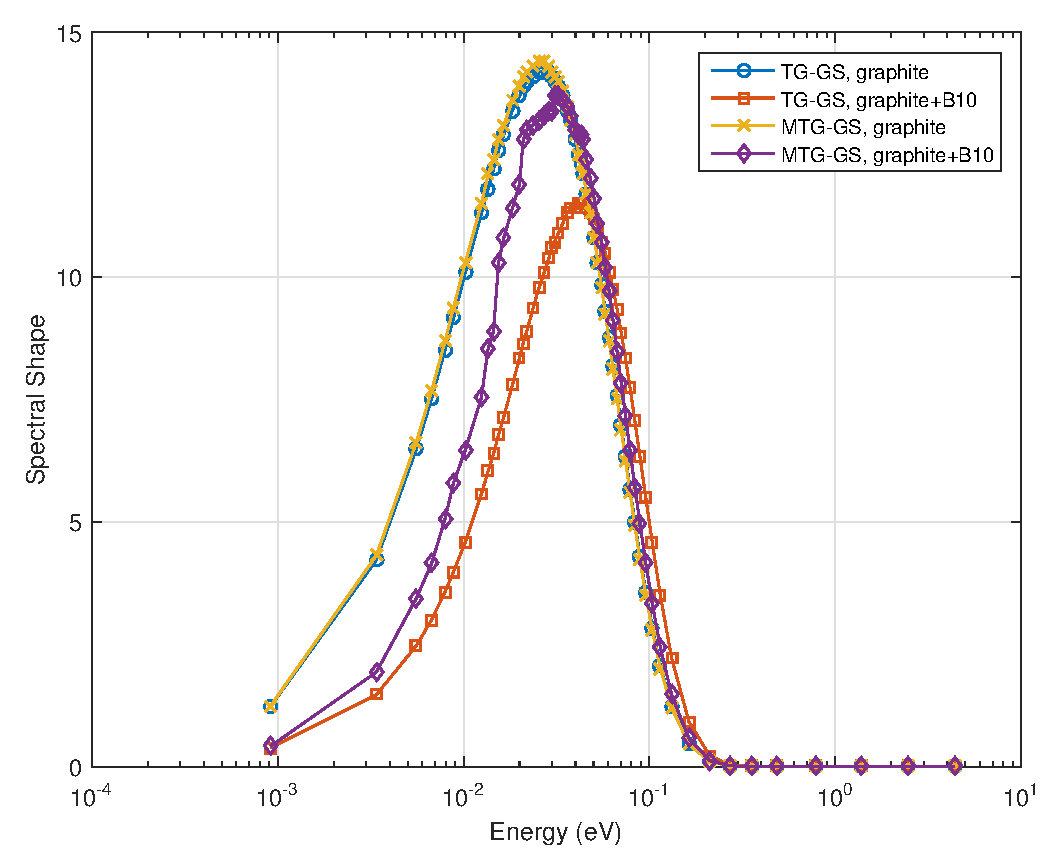
\includegraphics[width=0.85\textwidth]{figures/SS_GS_graphite.eps}
\caption{Spectral shapes of the Gauss-Seidel methods for pure graphite and graphite with 50 ppm of boron-10.}
\label{fig::Flat_FA_TGandMTG}
\end{figure}

\begin{figure}
\centering
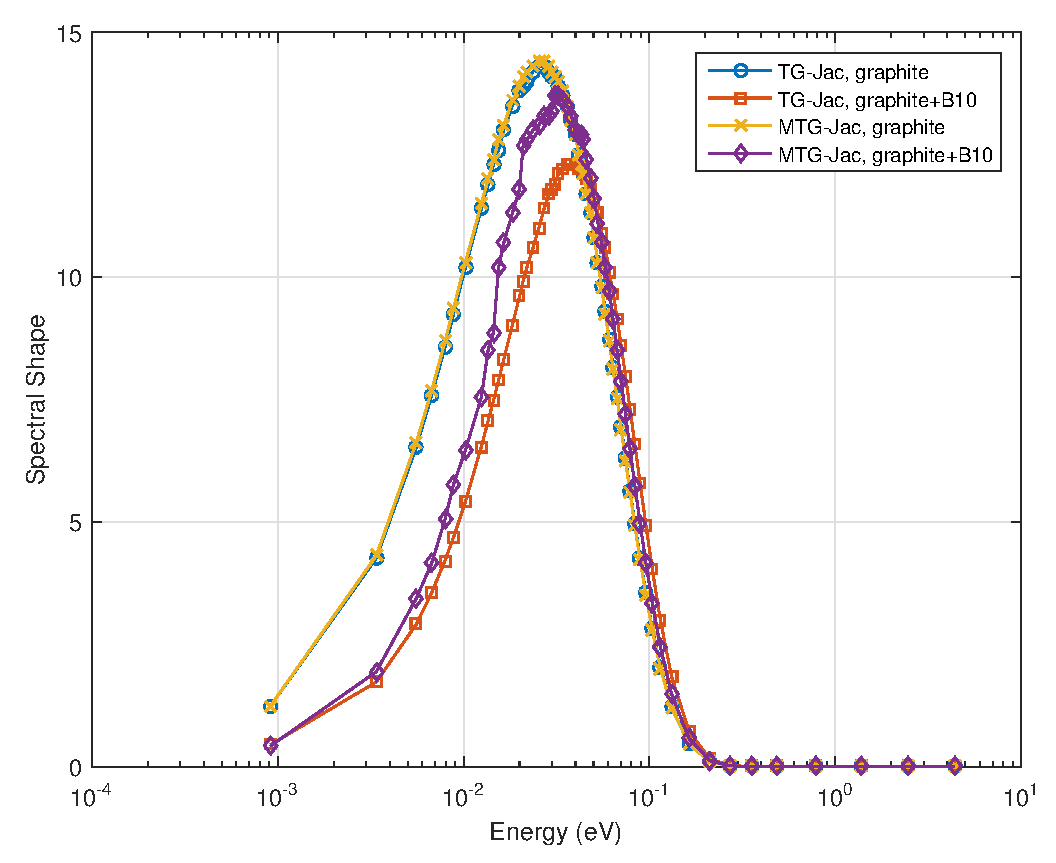
\includegraphics[width=0.85\textwidth]{figures/SS_Jac_graphite.eps}
\caption{Spectral shapes of the Jacobi methods for pure graphite and graphite with 50 ppm of boron-10.}
\label{fig::Flat_FA_TGandMTG}
\end{figure}
% ------------------------------

% Flat-mode eigenvalues
% ---------------------------
\begin{figure}
\centering
	\begin{subfigure}[b]{0.85\textwidth}
		\centering
		\includegraphics[width=0.975\textwidth]{\DSAfigpath{IM1_Graph_FA_TG.eps}}
		\caption{TG-GS Acceleration}
	\end{subfigure}
	
	\begin{subfigure}[b]{0.85\textwidth}
		\centering
		\includegraphics[width=0.975\textwidth]{\DSAfigpath{IM1_Graph_FA_MTG.eps}}
		\caption{MTG-GS Acceleration}
	\end{subfigure}
\caption{Flat mode eigenvalues for the TG-GS and MTG-GS schemes.}
\label{fig::Flat_FA_TGandMTG}
\end{figure}

\begin{figure}
\centering
	\begin{subfigure}[b]{0.85\textwidth}
		\centering
		\includegraphics[width=0.975\textwidth]{\DSAfigpath{IM1_Graph_FA_MJA.eps}}
		\caption{MTG-Jac Acceleration}
	\end{subfigure}
	
	\begin{subfigure}[b]{0.85\textwidth}
		\centering
		\includegraphics[width=0.975\textwidth]{\DSAfigpath{IM1_Graph_FA_MJIA.eps}}
		\caption{TG-Jac Acceleration}
	\end{subfigure}
\caption{Flat mode eigenvalues for the TG-Jac and MTG-Jac schemes.}
\label{fig::Flat_FA_MJAandMJIA}
\end{figure}
% ---------------------------

%------------------------------------------------------------------------------------------------------------
\subsection{Homogeneous Graphite Configuration}
%------------------------------------------------------------------------------------------------------------
\tcr{I was thinking a simple table with iteration statistics for a homogenous cube problem.}

\tcr{expectations: these results will match closely the FA results.}

The numerical spectral radius of each method (unaccelerated and accelerated) was estimated with the following:

\begin{equation}
\label{eq::MG_NSR_est}
\rho^{(k+1)} \approx \sqrt{\frac{\sum\limits_{g=1}^{G_{th}} \sum\limits_{K \in \mathcal{T}_h} \sum\limits_{i=1}^{N_K} \left(  \Phi_{g,K,i}^{(k+1)} - \Phi_{g,K,i}^{(k)} \right)^2}{\sum\limits_{g=1}^{G_{th}} \sum\limits_{K \in \mathcal{T}_h} \sum\limits_{i=1}^{N_K} \left(  \Phi_{g,K,i}^{(k)} - \Phi_{g,K,i}^{(k-1)} \right)^2}} ,
\end{equation}

\noindent where $\Phi_{g,K,i}^{(k)}$ is the $k$-iterate scalar flux for basis function $i$ of cell $K$ of thermal energy group $g$.

\begin{table}
\caption{Sweep count and timing data for the 2D IM1 variant problem using Two-Grid Acceleration.}
\centering
\def\arraystretch{1.25}
\begin{tabular}{|c|c|c|c|c|}
\hline
Acceleration Method & Outer Iter.  & 1-Group Sweeps & SR & NSR  \\
\hline \hline
None & 0 & 0 & 0 & \\ \hline
TG-GS & {361}  &{185,422}  &  {486.50} &\\ \hline
MTG-GS & 55 & 35,699 &  96.48 &\\ \hline
MTG-Jac & 38  & 41,575 &  128.63 & \\ \hline
TG-Jac & 14  & 19,053  & 57.92 & \\ \hline
\end{tabular}
\label{tab::IM1_2D_TG}
\end{table}

%------------------------------------------------------------------------------------------------------------
\subsection{Heterogeneous Configurations}
%------------------------------------------------------------------------------------------------------------

\tcr{2D and 3D IM1 results}

\tcr{make a note on the highly heterogeneous configuration for which it is well known that ``all'' diffusion based accelerator have trouble, see Warsa/Yaqi ``PHI''.}

% 2D results go here
% ---------------------

\begin{figure}
\centering
\includegraphics[width=0.65\textwidth]{\DSAfigpath{2D_IM1_Variant_Layout.png}}
\caption{Configuration of the 2D heterogeneous problem with air, HDPE, graphite, and AmBe source materials.}
\label{fig::IM1_config_2D}
\end{figure}

\begin{table}
\caption{Sweep count and timing data for the 2D IM1 variant problem using Two-Grid Acceleration.}
\centering
\def\arraystretch{1.25}
\begin{tabular}{|c|c|c|c|}
\hline
Problem & Outer Iter.  & 1-Group Sweeps & Solve Time (min)  \\
\hline \hline
{SI} & {361}  &{185,422}  &  {486.50} \\ \hline
SI+DSA & 55 & 35,699 &  96.48 \\ \hline
GMRES & 38  & 41,575 &  128.63 \\ \hline
GMRES+DSA & 14  & 19,053  & 57.92  \\ \hline
\end{tabular}
\label{tab::IM1_2D_TG}
%\end{table}
\vspace{1.5cm}
%\begin{table}
\caption{Sweep count and timing data for the 2D IM1 variant problem using Modified Two-Grid Acceleration.}
\centering
\def\arraystretch{1.25}
\begin{tabular}{|c|c|c|c|}
\hline
Problem & Outer Iter.  & 1-Group Sweeps & Solve Time (min)  \\
\hline \hline
{SI} & {536}  & {77,632} & {275.83}  \\ \hline
SI+DSA & 73  & 10,846 &  40.60 \\ \hline
GMRES & 78  & 4,845 &  25.82 \\ \hline
GMRES+DSA & 26  & 1,881 & 11.09  \\ \hline
\end{tabular}
\label{tab::IM1_2D_MTG}
%\end{table}
\vspace{1.5cm}
%\begin{table}
\caption{Sweep count and timing data for the 2D IM1 variant problem using Multigroup Jacobi Acceleration.}
\centering
\def\arraystretch{1.25}
\begin{tabular}{|c|c|c|c|}
\hline
Problem & Outer Iter.  & 1-Group Sweeps & Solve Time (min)  \\
\hline \hline
{SI}  & {1,734} & {98,838} &  {111.07} \\ \hline
SI+DSA  & 157 & 8,949 &  15.49 \\ \hline
GMRES  & 118 & 6,726 &  8.65 \\ \hline
{GMRES+DSA} &   {35} & {1,995} &  {4.16} \\ \hline
\end{tabular}
\label{tab::IM1_2D_MJA}
\end{table}

 % ---------------------

%%%%%%%%%%%%%%%%%%%%%%%%%%%%%%%%%%%%%%%%%%%%%%%%%%%%%%%%%%%%%%%%%%%%
%%%%%%%%%%%%%%%%%%%%%%%%%%%%%%%%%%%%%%%%%%%%%%%%%%%%%%%%%%%%%%%%%%%%
\section{Conclusions} \label{sec::conclusions}
%%%%%%%%%%%%%%%%%%%%%%%%%%%%%%%%%%%%%%%%%%%%%%%%%%%%%%%%%%%%%%%%%%%%
%%%%%%%%%%%%%%%%%%%%%%%%%%%%%%%%%%%%%%%%%%%%%%%%%%%%%%%%%%%%%%%%%%%%

In this paper,

%%%%%%%%%%%%%%%%%%%%%%%%%%%%%%%%%%%%%%%%%%%%%%%%%%%%%%%%%%%%%%%%%%%%
%%%%%%%%%%%%%%%%%%%%%%%%%%%%%%%%%%%%%%%%%%%%%%%%%%%%%%%%%%%%%%%%%%%%
\section*{Acknowledgments} 
%%%%%%%%%%%%%%%%%%%%%%%%%%%%%%%%%%%%%%%%%%%%%%%%%%%%%%%%%%%%%%%%%%%%
%%%%%%%%%%%%%%%%%%%%%%%%%%%%%%%%%%%%%%%%%%%%%%%%%%%%%%%%%%%%%%%%%%%%
This research was performed under appointment to the Rickover Graduate Fellowship Program in Nuclear Engineering sponsored by the Naval Reactors Division of the United States Department of Energy.

%%%%%%%%%%%%%%%%%%%%%%%%%%%%%%%%%%%%%%%%%%%%%%%%%%%%%%%%%%%%%%%%%%%%
%%%%%%%%%%%%%%%%%%%%%%%%%%%%%%%%%%%%%%%%%%%%%%%%%%%%%%%%%%%%%%%%%%%%
%%%%%%%%%%%%%%%%%%%%%%%%%%%%%%%%%%%%%%%%%%%%%%%%%%%%%%%%%%%%%%%%%%%%
%%%%%%%%%%%%%%%%%%%%%%%%%%%%%%%%%%%%%%%%%%%%%%%%%%%%%%%%%%%%%%%%%%%%
\bibliographystyle{elsarticle-num}
\bibliography{references}

% Begin appendices
\appendix
%%%%%%%%%%%%%%%%%%%%%%%%%%%%%%%%%%%%%%%%%%%%%%%%%%%%%%%%%%%%%%%%%%%%
%%%%%%%%%%%%%%%%%%%%%%%%%%%%%%%%%%%%%%%%%%%%%%%%%%%%%%%%%%%%%%%%%%%%
\section{Bilinear Form of the Modified Interior Penalty Method}  \label{app::mip}
%%%%%%%%%%%%%%%%%%%%%%%%%%%%%%%%%%%%%%%%%%%%%%%%%%%%%%%%%%%%%%%%%%%%
%%%%%%%%%%%%%%%%%%%%%%%%%%%%%%%%%%%%%%%%%%%%%%%%%%%%%%%%%%%%%%%%%%%%

We write the MIP diffusion form as

\begin{equation}
a^{MIP}( b, \delta \Phi) = b^{MIP}(b),
\label{eq::MIP_weak_form}
\end{equation}

\noindent with the following bilinear matrix,

\begin{equation}
\label{eq::MIP_bilinear_form}
\begin{aligned}
a^{MIP}(b, \delta \Phi)  = \Big(  D \vec{\nabla} b , \vec{\nabla} \delta \Phi  \Big)_{\mathcal{D}} + \Big(  \sigma b , \delta \Phi  \Big)_{\mathcal{D}}    \\
+  \Big< \kappa_f^{MIP} [\![   b ]\!] , [\![  \delta \Phi ]\!]\Big>_{E_h^i} + \Big<  [\![  b ]\!] , \{\!\{  D \partial_n \delta \Phi \}\!\}\Big>_{E_h^i}  + \Big< \{\!\{  D \partial_n b \}\!\} , [\![ \delta \Phi ]\!]\Big>_{E_h^i} \\
+ \Big< \kappa_f^{MIP}  b , \delta  \Phi \Big>_{\partial \mathcal{D}^d} - \frac{1}{2} \Big<  b ,  D \partial_n \delta \Phi \Big>_{\partial \mathcal{D}^d} - \frac{1}{2} \Big<   D \partial_n b , \delta \Phi \Big>_{\partial \mathcal{D}^d}  
\end{aligned} ,
\end{equation}

\noindent and with the following linear right-hand-side,

\begin{equation}
\label{eq::MIP_linear_form}
b^{MIP} (b) = \Big(  b, Q  \Big)_{\mathcal{D}}  + \Big< b, \delta  J^{inc}  \Big>_{\partial \mathcal{D}^{ref}} .
\end{equation}

\noindent  The mean value and the jump terms in Eq. (\ref{eq::MIP_bilinear_form}) are given by

\begin{equation}
\label{eq::solution_mean_and_jump}
\{\!\{  \Phi \}\!\} \equiv \frac{\Phi^+ + \Phi^-}{2} \qquad \text{and} \qquad [\![   \Phi ]\!] \equiv \Phi^+ - \Phi^- ,
\end{equation}

\noindent respectively. The directionality of the terms across a face can be defined in negative, $\Phi^-$, and positive, $\Phi^+$ directions by their trace:

\begin{equation}
\label{eq::solution_trace}
\Phi^{\pm} \equiv \lim_{s \rightarrow 0^{\pm}} \Phi (\vec{r} + s \vec{n}),
\end{equation}

\noindent where the face's unit normal direction, $\vec{n}$ is arbitrarily chosen for interior faces and outwards for boundary faces. The penalty coefficient, $\kappa_f^{MIP}$, is face-dependent and its functional form is given by

\begin{equation}
\label{eq::MIP_penalty_term}
\kappa_f^{MIP} = \text{max} \left( \kappa_f^{IP}, \frac{1}{4} \right) ,
\end{equation}

\noindent where

\begin{equation}
\label{eq::SIP_penalty_term}
\kappa_f^{IP} = 
\begin{cases}
	\frac{c}{2} \left(  \frac{D^+}{h^+} + \frac{D^-}{h^-} \right) & f \in E_h^i\\ 
	c \frac{D^-}{h^-}& f \in \partial \mathcal{D}
\end{cases}.
\end{equation}

\noindent In Eq. (\ref{eq::SIP_penalty_term}), $D^{\pm}$ and $h^{\pm}$ correspond to the diffusion coefficient and orthogonal projections, respectively, on either side of a face. The orthogonal projection is defined as the length of a face orthogonally projected into the mesh cell. Turcksin and Ragusa, \cite{turcksin2014discontinuous}, defined $h^\pm$ for 2D polygons, whose definitions can be seen in Table \ref{tab::orth_proj_2D}.

\begin{table}[h]
\centering
\caption{Orthogonal projection, $h$, for different polygonal types: $A_K$ is the area of cell $K$, $L_f$ is the length of face $f$, and $P_K$ is the perimeter of cell $K$.}
\def\arraystretch{1.4}
\begin{tabular}{|c|c|c|c|c|}
	\hline
	Number of Vertices & 3 & 4 & $>4$ and even& $>4$ and odd \\
	\hline
	$h$ & $2 \frac{A_K}{L_f}$ & $\frac{A_K}{L_f}$ & $4 \frac{A_K}{P_K}$ & $2 \frac{A_K}{P_K} + \sqrt{\frac{2 A_K}{N_K \sin(\frac{2 \pi}{N_K})}}$ \\
	\hline
\end{tabular}
\label{tab::orth_proj_2D}
\end{table}

\end{document}
